\section{Akurasi Implementasi \acl{RL}}

Terdapat dua metode yang diajukan sebagai \textit{improvement} komputasi \ac{RL} pada penelitian ini: algoritma \ref{alg:rl-qmemo} yang mampu melakukan memoisasi agar memperbaik hasil komputasi \ac{RL} dan akselerator perangkat keras. Hasil uji akurasi terhadap kedua metode ini akan dibahas pada sub subbab selanjutnya.


% TODO: bikin bar chart untuk hasil comparison software dan hardware
\section{Akurasi Implementasi Algoritma \ref{alg:rl-qmemo} pada Perangkat Lunak}

Pengujian akurasi algoritma \ref{alg:rl-qmemo} dilakukan dengan pembandingan hasil akhir yang didapat dari algoritma tersebut dengan implementasi \ac{DFS}. Kedua algoritma dibandingkan hasil jalur tercepatnya dari labirin berdimensi 2 sampai 10 yang dihasilkan dari algoritma Prim pada \ref{alg:prim}. Gambar \ref{fig:akurasi-qmemo} memperlihatkan hasil plot dari variasi dimensi labirin terhadap banyak langkah yang diambil pada labirin untuk menyelesaikannya.

\begin{figure}[h]
	\centering
	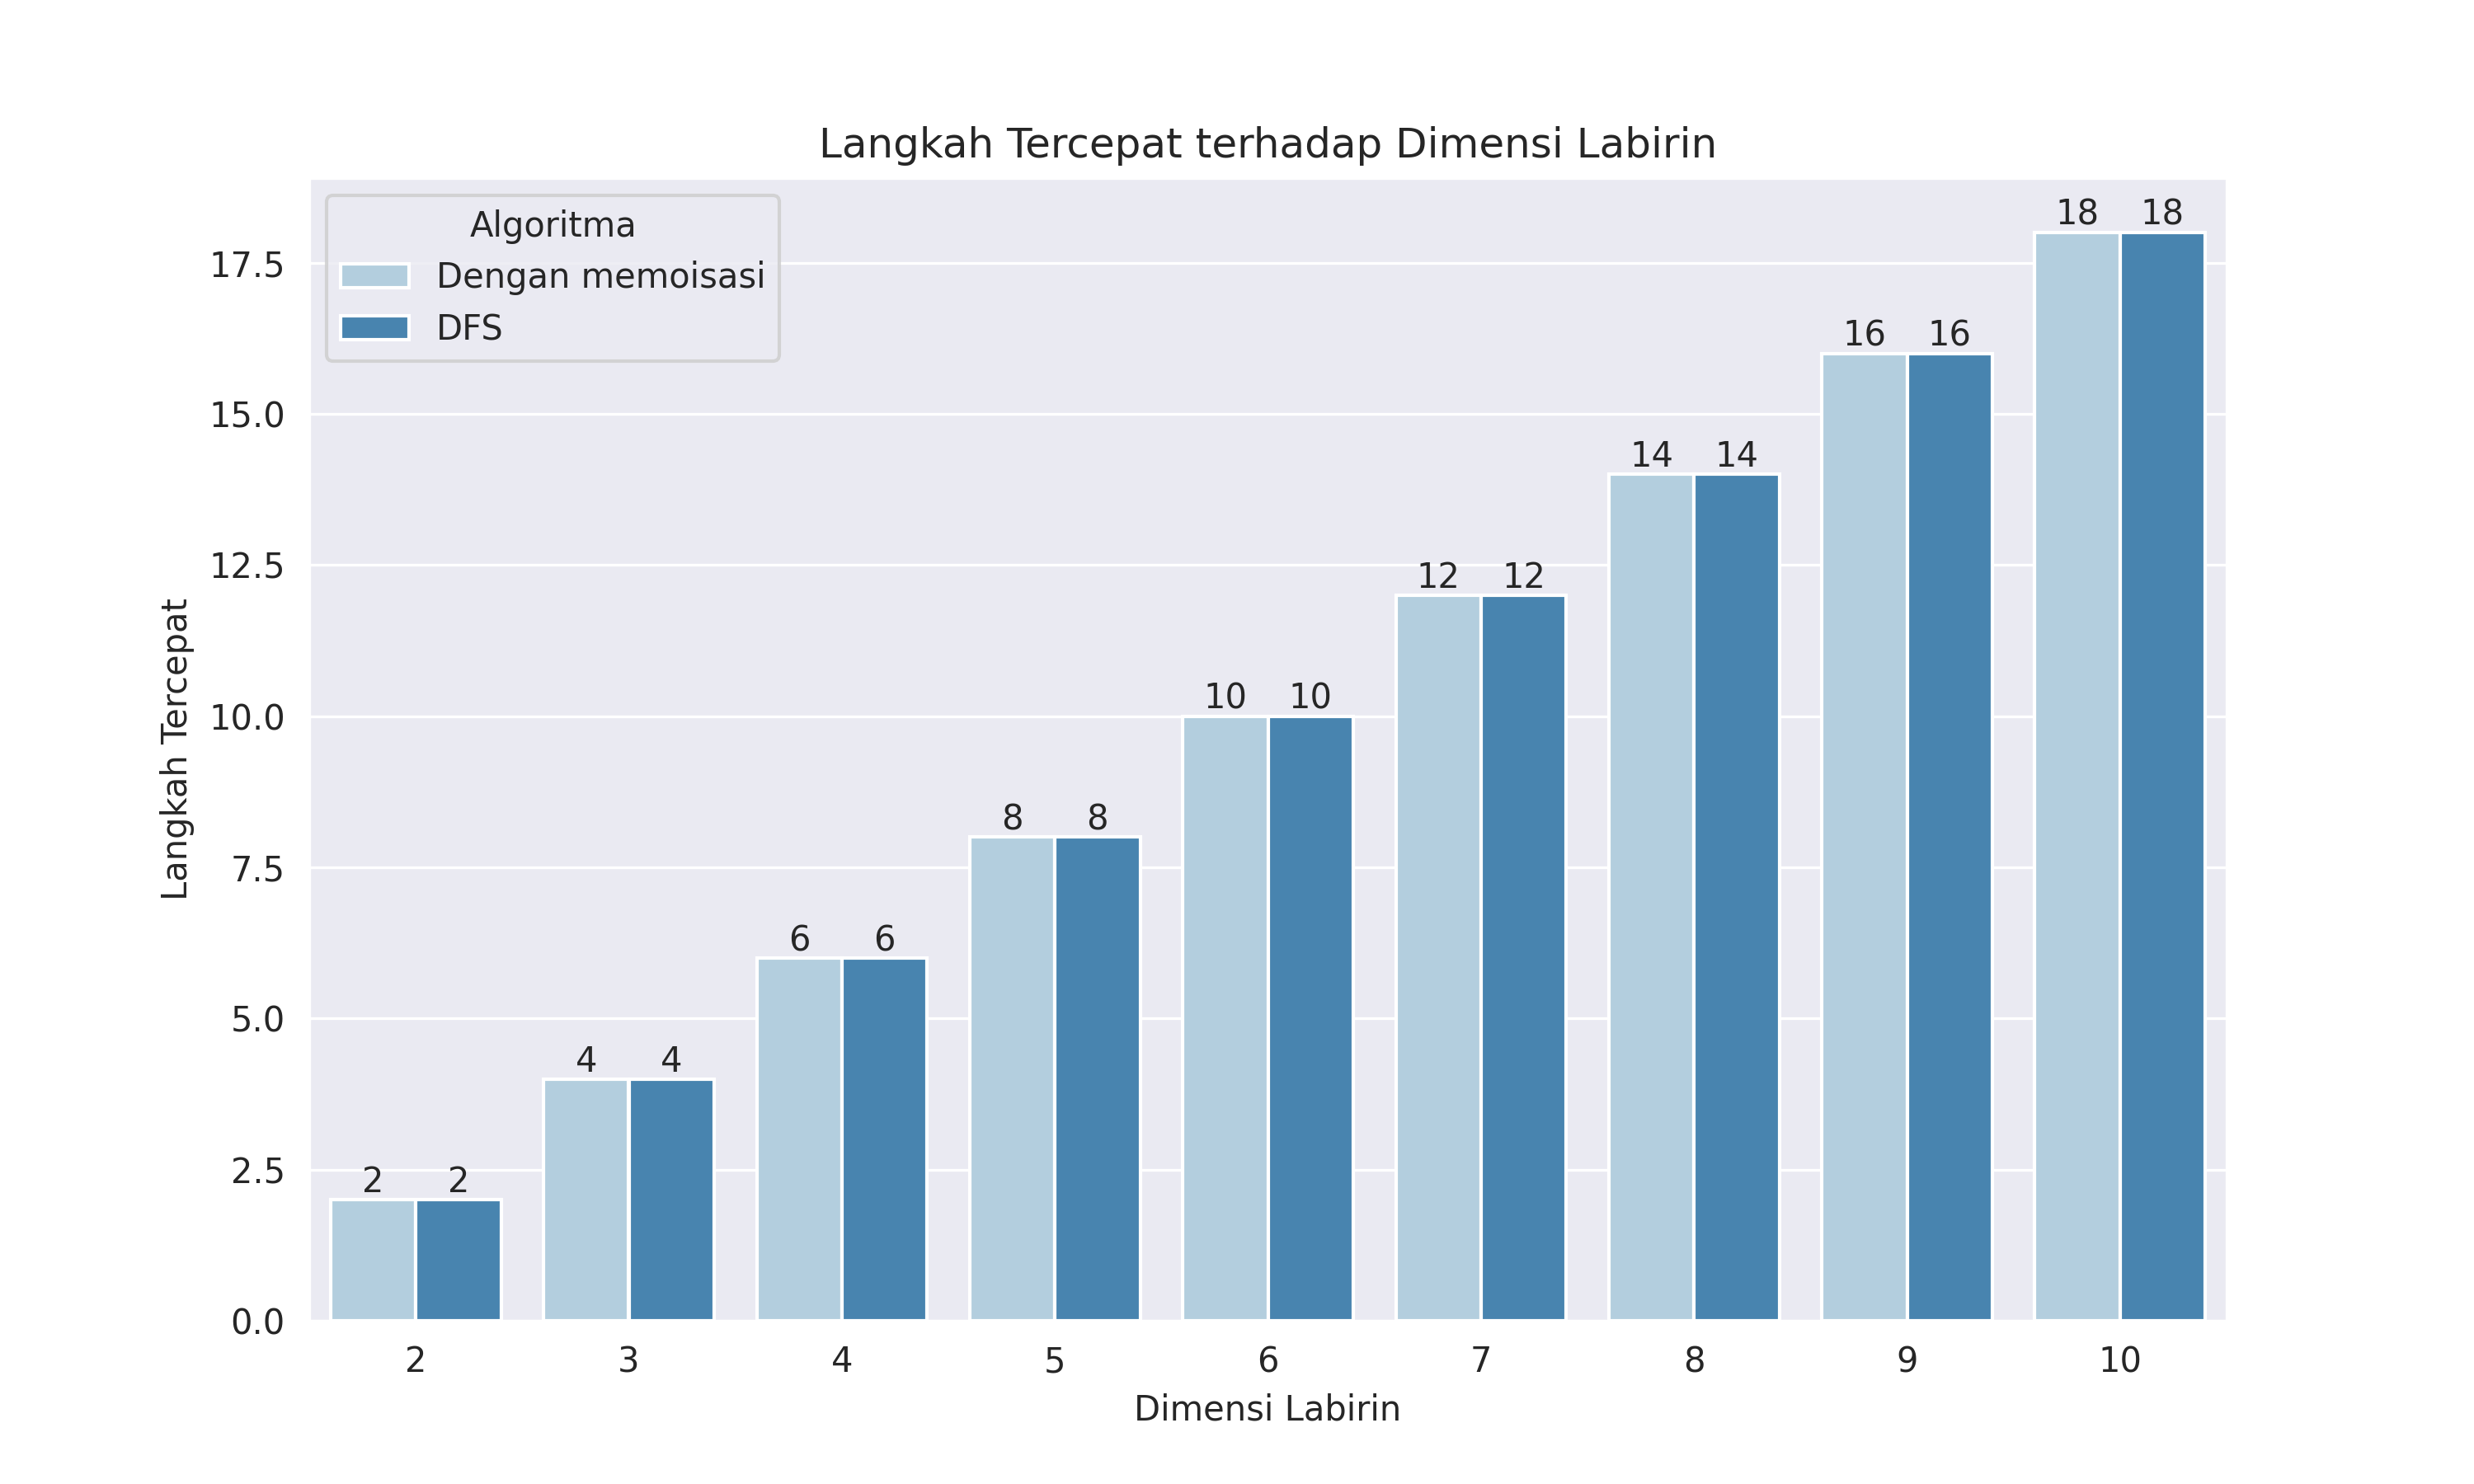
\includegraphics[width=1\textwidth]{chapter-4/plot-akurasi-qmemo.png}
	\caption{Hasil pengujian akurasi algoritma \ref{alg:rl-qmemo}}
	\label{fig:akurasi-qmemo}
\end{figure}

Gambar \ref{fig:akurasi-qmemo} menunjukkan bahwa agen \ac{RL} dapat melakukan pembelajaran secara baik karena dapat menghasilkan nilai tempuh yang optimal sesuai dengan hasil dari \ac{DFS}. Selanjutnya, dilakukan perbandingan \textit{cumulative rewards} yang didapatkan dari hasil pembelajaran agen \ac{RL} dari algoritma konvensional \ref{alg:rl-qlearning} dan dengan memoisasi \ref{alg:rl-qmemo}. Konfigurasi yang digunakan untuk pengujian ini dilakukan untuk memperlihatkan efektifitas algoritma \ref{alg:rl-qmemo} dengan menyelesaikan masalah labirin dengan dimensi 20 dan 40. Dimensi tersebut dipilih agar dapat merepresentasikan contoh kasus dalam posibilitas \textit{state} yang banyak. Gambar \ref{fig:memo-result} merupakan hasil plot dari pengujian tersebut.

\begin{figure}[h]
	\centering
	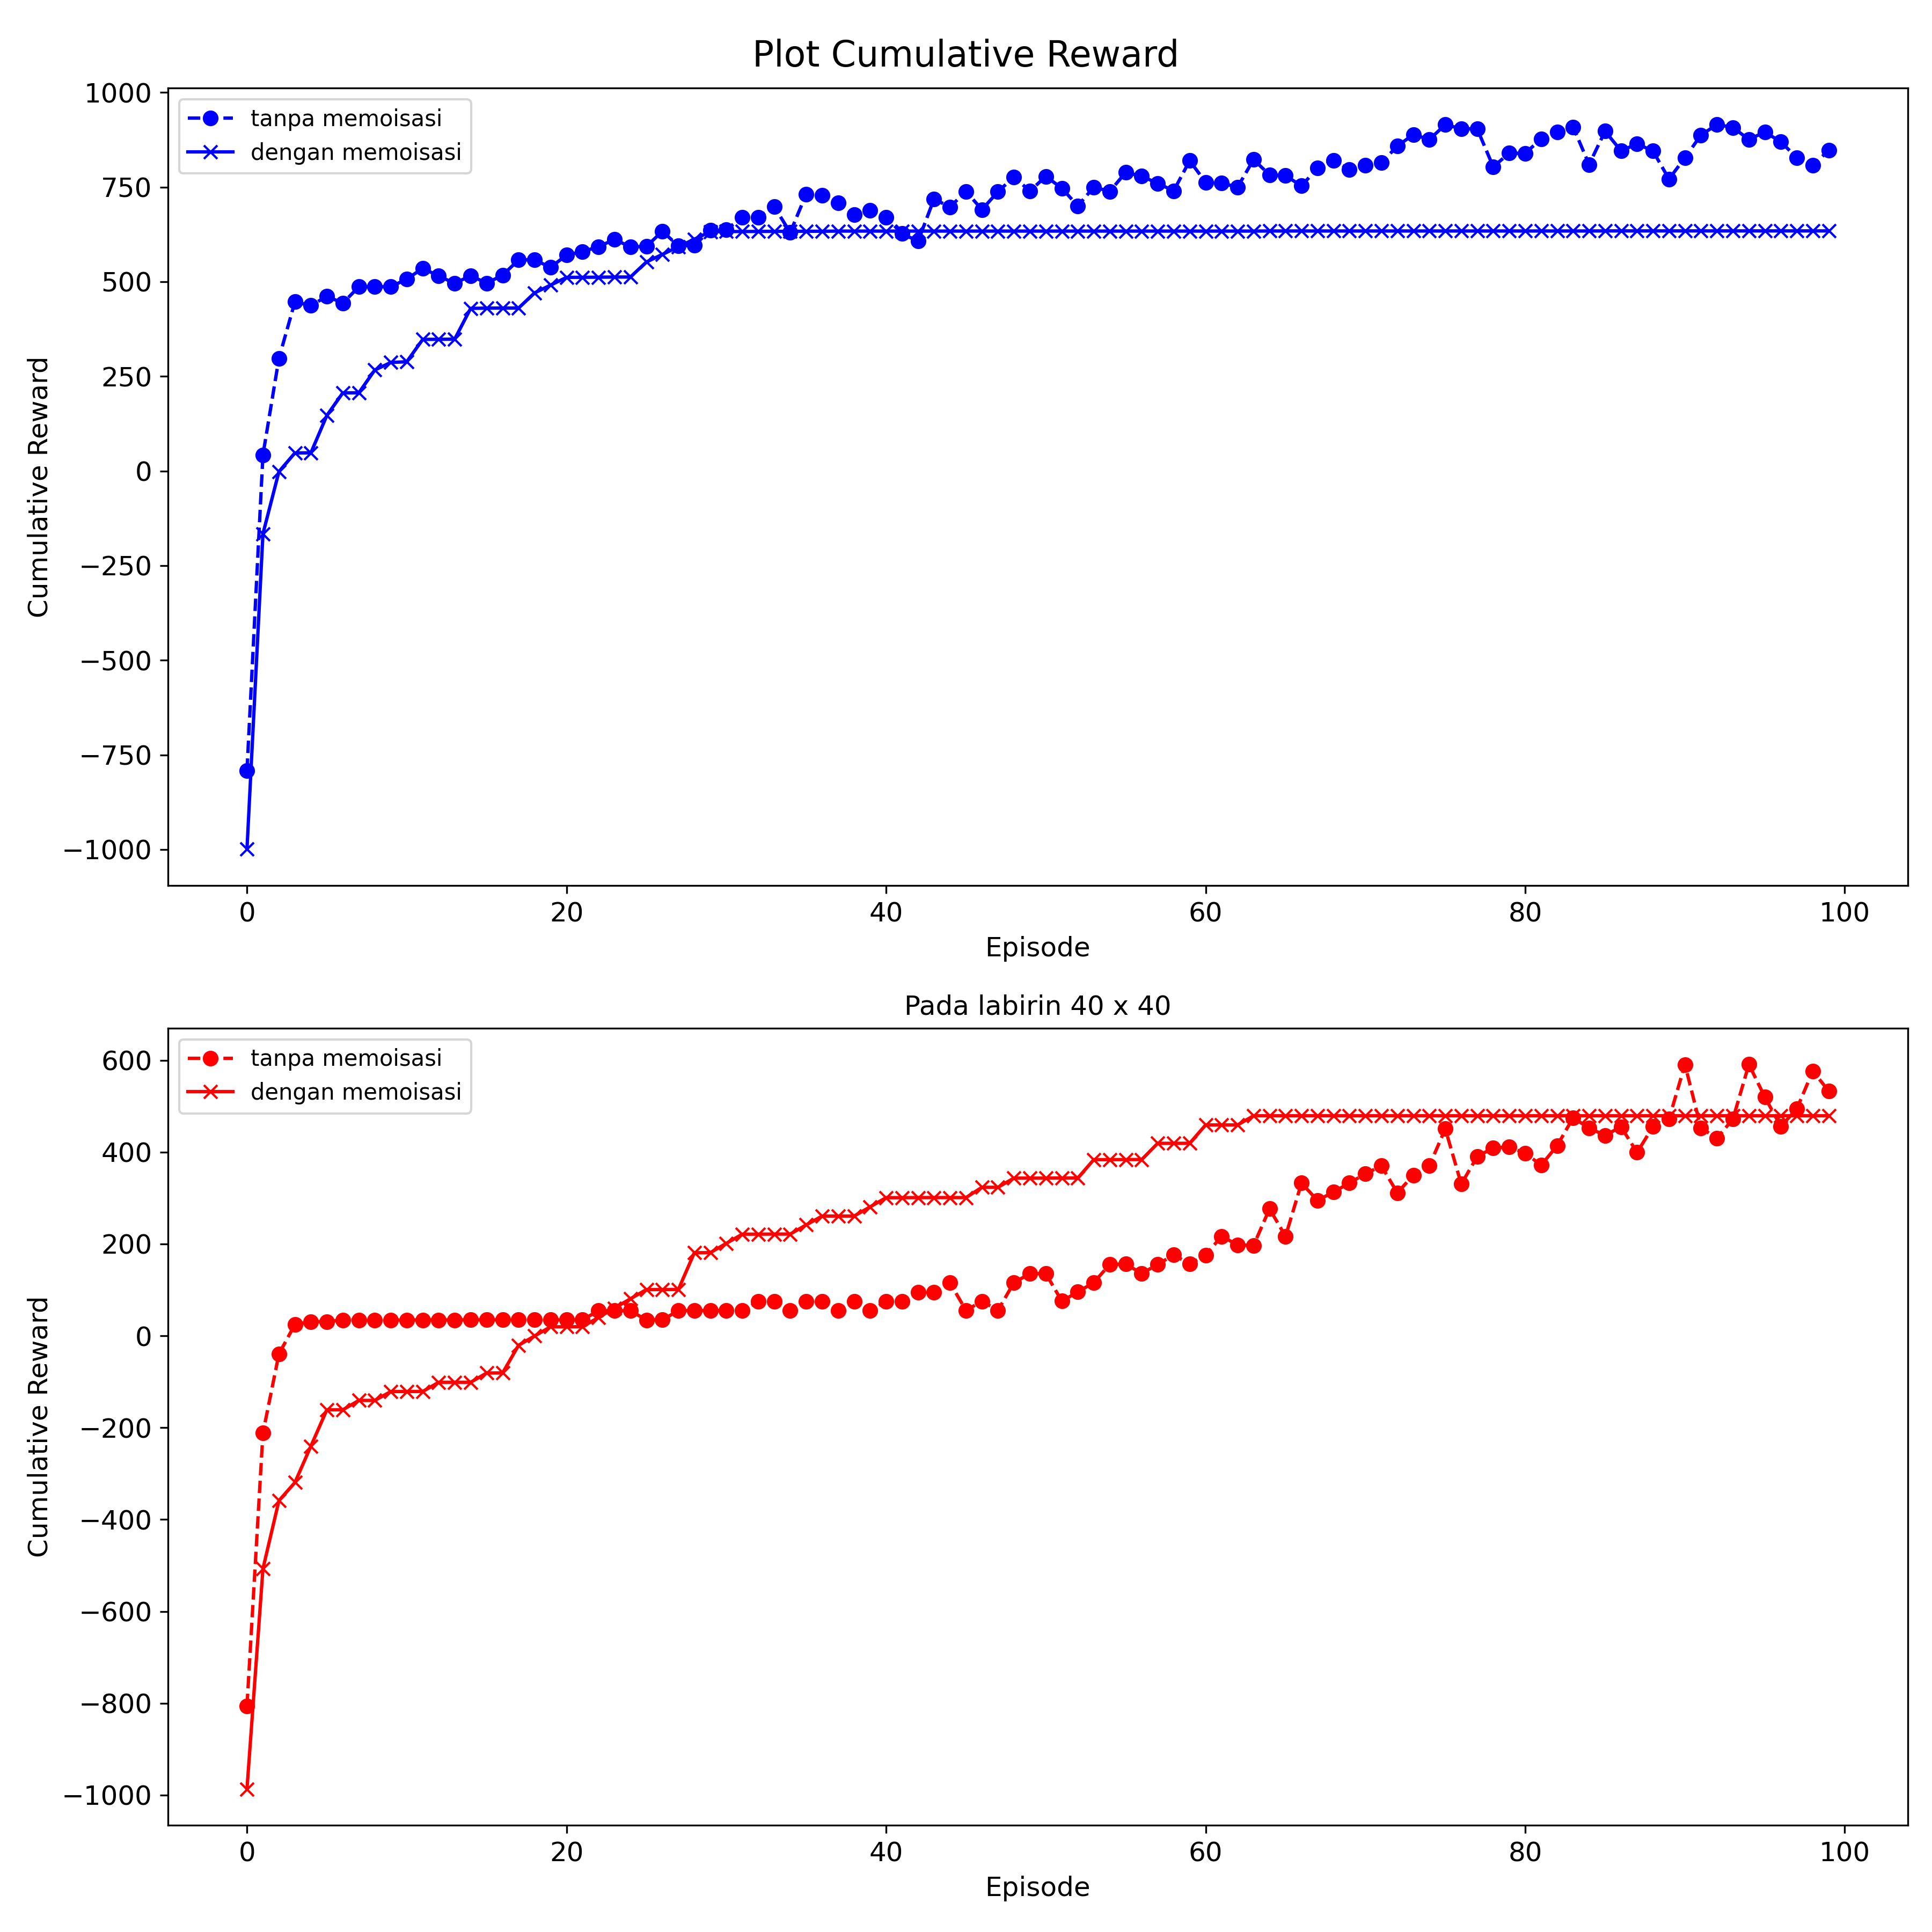
\includegraphics[width=1\textwidth]{chapter-4/memo-result.png}
	\caption{Hasil pengujian algoritma \ref{alg:rl-qmemo}}
	\label{fig:memo-result}
\end{figure}

Hasil pada gambar \ref{fig:memo-result} memperlihatkan bahwa algoritma \ref{alg:rl-qmemo} memiliki konsistensi lebih baik dibanding kepada algoritma konvensional yang digunakan pada algoritma \ref{alg:rl-qlearning}. Namun, algoritma \ref{alg:rl-qmemo} memiliki kekurangan yaitu terkadang lambat untuk mempelajari alternatif $\pi^*$ yang optimal. Sehingga, algoritma ini baik untuk digunakan pada kasus dimana perubahan \textit{cumulative reward} yang sedikit akan berpengaruh secara besar. Contoh dari kasus tersebut adalah kasus \textit{reinforcement learning} yang menggunakan aksi diskrit seperti permasalahan labirin pada penelitian ini.

\section{Akurasi Implementasi pada Akselerator}

Pengujian akurasi akselerator dilakukan menggunakan setup seperti digambarkan pada sub sub-bab \ref{subsec:verilator}. Pengujian akurasi dilakukan untuk seluruh instruksi dengan konfigurasi dan hasil \textit{timing diagram} pada lampiran \ref{appendix:verilator}. Hasil pada lampiran \ref{appendix:verilator} menunjukkan bahwa implementasi akselerator memiliki akurasi 100\% sesuai dengan implementasi dari perangkat lunak.
